% !TEX root = ../ds3.tex


%%%%%%%%%%%%%%%%%%%%%%%%%%%%%%%%%%%%%%%%%%%%%%%%%%%%%%%%%%%%%%%%%%%%%%%%%%%%%%%
%%%%%%%%%%%%%%%%%%%%%%%%%%%%%%%%%%%%%%%%%%%%%%%%%%%%%%%%%%%%%%%%%%%%%%%%%%%%%%%
\section{Gradient descent}
%%%%%%%%%%%%%%%%%%%%%%%%%%%%%%%%%%%%%%%%%%%%%%%%%%%%%%%%%%%%%%%%%%%%%%%%%%%%%%%
%%%%%%%%%%%%%%%%%%%%%%%%%%%%%%%%%%%%%%%%%%%%%%%%%%%%%%%%%%%%%%%%%%%%%%%%%%%%%%%


%%%%%%%%%%%%%%%%%%%%%%%%%%%%%%%%%%%%%%%%%%%%%%%%%%%%%%%%%%%%%%%%%%%%%%%%%%%%%%%
\begin{frame}{One framework to rule them all: surrogate minimization}
    \alert{Taylor expansion}
    \begin{align*}
        f(w)
        \leq
        \underbrace{f(w^{k})
        + \langle \nabla f (w^{k}), w - w^{k} \rangle
        + \frac{L}{2} \normin{w - w^{k}}^2}_{\text{Surrogate function } \tilde{f}(w)}
    \end{align*}

    \pause

    The \alert{surrogate} is minimized.
    $\tilde{f}$ is convex differentiable, infinite at the infinite (coercive), its minimum $w^*$ is achieved where gradient is 0:

    \begin{align*}
        0 = \nabla \tilde{f} (w^*) = \nabla f (w^{k}) + L (w^* - w^{k})
    \end{align*}

    \pause
    Taking $w^{k+1}$ as the minimizer of $\tilde{f}$ leads to \alert{gradient descent}:

    \begin{align*}
        w^{k+1} = w^k - \frac{1}{L} \nabla f (w^k)
    \end{align*}
\end{frame}
%%%%%%%%%%%%%%%%%%%%%%%%%%%%%%%%%%%%%%%%%%%%%%%%%%%%%%%%%%%%%%%%%%%%%%%%%%%%%%%


%%%%%%%%%%%%%%%%%%%%%%%%%%%%%%%%%%%%%%%%%%%%%%%%%%%%%%%%%%%%%%%%%%%%%%%%%%%%%%%
\begin{frame}{Example of GD}
    \centering
    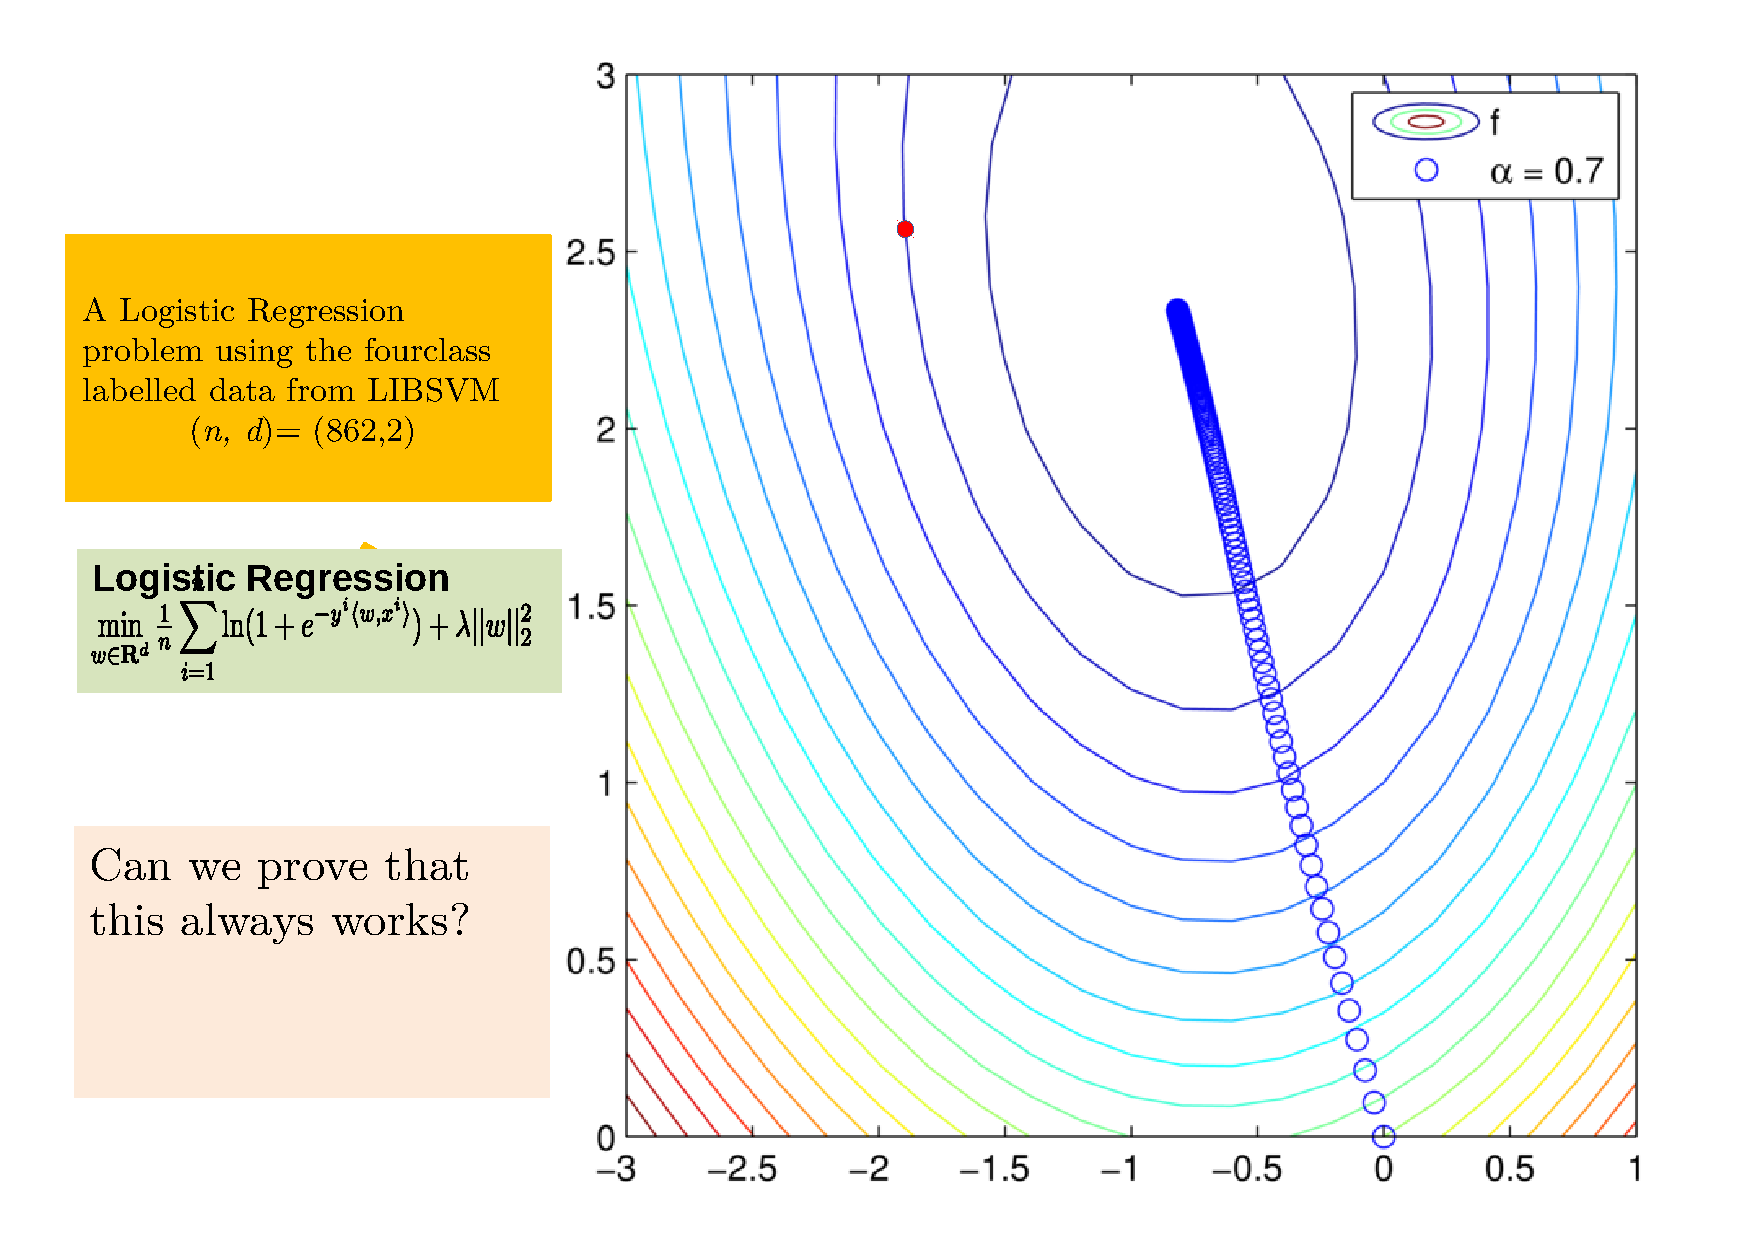
\includegraphics[width=30em]{graident_descent}

    Gradient descent on a 2D problem
\end{frame}
%%%%%%%%%%%%%%%%%%%%%%%%%%%%%%%%%%%%%%%%%%%%%%%%%%%%%%%%%%%%%%%%%%%%%%%%%%%%%%%

%%%%%%%%%%%%%%%%%%%%%%%%%%%%%%%%%%%%%%%%%%%%%%%%%%%%%%%%%%%%%%%%%%%%%%%%%%%%%%%
\begin{frame}{Line-search \footfullcite[Chap. 3]{Nocedal_Wright06}}
    What to do when a function is smooth, but you do not know the Lipschitz constant $L$? Or when $L$ is too conservative?

    \pause
    %
    Gradient descent with variable stepsize:
    %
    \begin{align*}
        w^{k+1} = w^k - \alpha^k \nabla f (w^k)
    \end{align*}
    where the stepsize $\alpha$ changes at each iteration
\end{frame}
%%%%%%%%%%%%%%%%%%%%%%%%%%%%%%%%%%%%%%%%%%%%%%%%%%%%%%%%%%%%%%%%%%%%%%%%%%%%%%%

%%%%%%%%%%%%%%%%%%%%%%%%%%%%%%%%%%%%%%%%%%%%%%%%%%%%%%%%%%%%%%%%%%%%%%%%%%%%%%%
\begin{frame}{lab0 'gradient descent line-search'}
    Your turn!

    \begin{itemize}
        \item  Play with the gradient descent to gain insight!
    \end{itemize}

\end{frame}
%%%%%%%%%%%%%%%%%%%%%%%%%%%%%%%%%%%%%%%%%%%%%%%%%%%%%%%%%%%%%%%%%%%%%%%%%%%%%%%


%%%%%%%%%%%%%%%%%%%%%%%%%%%%%%%%%%%%%%%%%%%%%%%%%%%%%%%%%%%%%%%%%%%%%%%%%%%%%%%
\begin{frame}{Gradient descent: theoretical results}
    \begin{algorithm}[H]
        \SetKwInOut{Input}{input}
        \SetKwInOut{Init}{init}
        \SetKwInOut{Parameter}{param}
        \caption{GD}
        \Init{$w^0 = 0_{p}$, $L$}
            \For{$\mathrm{iter} =1,\dots,$}
                {
                $w^{k+1} = w^k - \frac{1}{L} \nabla f (w^k)$
                }
    % \Return{$w^{}$}
    \end{algorithm}
    %
    \pause
    %
    \begin{proposition}[TODO find ref]
        If $f$ is convex and $L$-smooth, then:
        \[
        f(w^{k}) - f(w^*)
        \leq
        \frac{2 L \norm{w^0 - w^*}^2}{k}
        \]
    \end{proposition}
    %
    \pause
    %
    \begin{proposition}[TODO find ref]
        If $f$ is $\mu$-strongly convex and $L$-smooth, then:
        \[
        \normin{w^{k} - w^*}
        \leq
        \left (
            1 - \frac{\mu}{L}
        \right)^k
        \]
    \end{proposition}
\end{frame}
%%%%%%%%%%%%%%%%%%%%%%%%%%%%%%%%%%%%%%%%%%%%%%%%%%%%%%%%%%%%%%%%%%%%%%%%%%%%%%%

%%%%%%%%%%%%%%%%%%%%%%%%%%%%%%%%%%%%%%%%%%%%%%%%%%%%%%%%%%%%%%%%%%%%%%%%%%%%%%%
\begin{frame}{Exercise: lab1 'logistic gd'}
    Your turn!

    \begin{itemize}
        \item  Play with the gradient descent to gain insight!
        \item Modify the code to take into account a regularization term
    \end{itemize}

    \vspace{2em}

    Reminders!
    \begin{itemize}
        \item In all the labs the main algorithm is already coded, and we propose you to add little modifications
        \item All the solutions are in the solutions folder
    \end{itemize}
\end{frame}
%%%%%%%%%%%%%%%%%%%%%%%%%%%%%%%%%%%%%%%%%%%%%%%%%%%%%%%%%%%%%%%%%%%%%%%%%%%%%%%
